\documentclass{article}

\title{Project - Cell Tracking}
\author{Arno Vermote - 01806792 \\
Arnoud De Jonge - 01808870 \\
Ewout Vlaeminck - 01801909 \\\\
Beeldverwerking [E010310A] - Universiteit Gent}
\date{11 december 2021}
\usepackage[utf8]{inputenc}
\usepackage{csquotes}
\usepackage[dutch]{babel}
\usepackage{multicol}
\setlength{\columnsep}{5mm} %column separation
\usepackage{graphicx}
\usepackage{biblatex}
\bibliography{references.bib}
\usepackage{wrapfig}
\usepackage{caption}
\usepackage[dutch]{hyperref}
\usepackage{floatrow}
\usepackage{titlesec}
\usepackage{floatrow}
\usepackage{amsmath}
\usepackage{enumitem}
\setlist{leftmargin=4.5mm}
\usepackage{xcolor} %for colour of font

%% Aanzetten als plaats tekort! %%
%\usepackage{setspace} %set for space between line
%\doublespacing %set for space between line
%%set page layout
%\titlespacing*{\section}
%{0pt}{0ex plus 1ex minus .2ex}{0ex plus .2ex}
%\titlespacing*{\subsection}
%{0.5pt}{0.5ex plus 1ex minus .2ex}{0.5ex plus .2ex}

\usepackage{titlesec}
\setcounter{secnumdepth}{4}
\titleformat{\paragraph}
{\normalfont\normalsize\bfseries}{\theparagraph}{1em}{}
\titlespacing*{\paragraph}
{0pt}{3.25ex plus 1ex minus .2ex}{1.5ex plus .2ex} % TODO title spacing aanpassen indien we plaats tekort hebben
\usepackage{geometry}
\geometry{
a4paper,
total={170mm,257mm},
left=20mm,
top=20mm,
}

 % TODO: zet een disclaimer dat alle afbeeldingen in HD apart in een mapje verkrijgbaar zijn ofzo
 % TODO: iets minder wikipedia refereren??
 % TODO: layout

\begin{document}
\maketitle

\begin{abstract}
In dit verslag onderzoeken we hoe we best de beweging volgen van cellen op microscoopbeelden. We bestuderen hiervoor voor iedere deelopdracht veschillende algoritmen. Voor celherkenning vergelijken we Features from Accelerated Segment Test, Laplacian of Gaussian, Difference of Gaussians en Determinant of the Hessian. Voor optische flow vergelijken we Horn-Schunck en Lucas-Kanade. Vervolgens combineren we de beste methode van iedere deelopdracht: Difference of Gaussians en Lucas-Kanade. Met dit resultaat zijn we in staat om accuraat cellen te volgen over meerdere beelden, gegeven de verwachte diameter van de cellen.

\end{abstract}

\begin{multicols}{2}

\section{Celherkenning}
De eerste voorwaarde voor het volgen van cellen is het detecteren welke pixels een cel voorstellen. Hiervoor bestaan verschillende methoden. We proberen enkelen en zullen de parameters van de methoden optimaliseren. Vervolgens vergelijken we de resultaten met elkaar en met reeds bestaande software: CellProfiler \cite{cell_profiler_org}.
De testset die in dit onderdeel gebruikt wordt, bestaat uit 4 opnames van de volledige dataset: A2, B2, C2 en D1.
Merk op dat in onze data een schaal rechts onderaan staat. Deze zullen we wegfilteren.

\subsection{Features from Accelerated Segment Test (FAST)}
\label{sec:fast}
Als eerste poging proberen we FAST\cite{ref_fast}, een randdetectie-algoritme. Deze methode werkt echter niet goed voor onze dataset: cellen die dicht of op elkaar liggen worden gedetecteerd als één grote cel. Ook zullen de celranden meerdere keren gedetecteerd worden. Hierdoor is bepalen welke pixel bij welke cel hoort niet triviaal doordat ze heel vaak overlappen. \autoref{fig:FAST} is een resultaat van deze methode, waar we de gedetecteerde randen in het blauw aanduiden.

\begin{figure}[H]
\centering
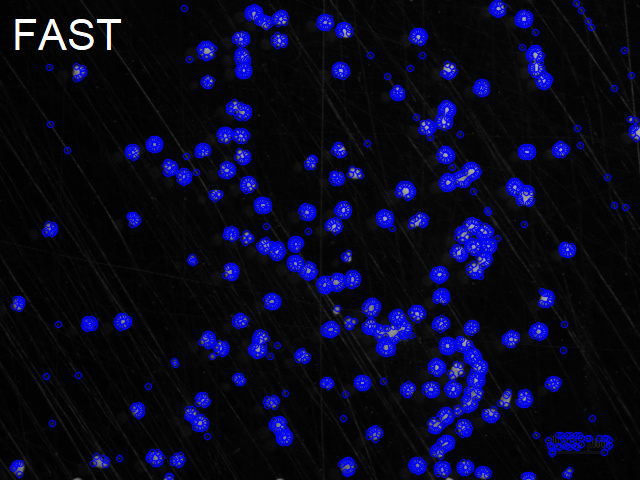
\includegraphics[width=0.98\textwidth]{images/fast_true.png}
\caption{\label{fig:FAST}FAST toegepast op één willekeurige frame van de data}
\end{figure}

Het is duidelijk dat deze methode niet goed werkt, zelfs niet met verschillende parameters. We zullen daarom deze ook niet gebruiken.

\subsection{Blobdetectie}
We zullen hier drie verschillende methoden voor blobdetectie toepassen en vergelijken: Laplacian of Gaussian (LoG) \cite{ref_log}, Difference of Gaussians (DoG) \cite{ref_dog} en Determinant of the Hessian (DoH) \cite{ref_doh}.

Voor deze technieken nemen we aan dat cellen ongeveer rond zijn. Hierdoor zullen we geen preciese randdetectie doen zoals in \autoref{sec:fast},  maar gewoon cirkels tekenen. Een voordeel hiervan is zichtbaar in de \autoref{fig:rand_vs_cirkel_detectie}: geclusterde cellen zullen niet als één grote cel gedetecteerd worden. Dit zal de precisie van het aantal gedetecteerde cellen verhogen. Dit probleem zien we ook bij CellTracker: er worden steeds minder cellen gedetecteerd dan er aanwezig zijn. Een nadeel van deze strategie is dat de vorm en grootte van cellen niet nauwkeurig weergegeven wordt.
\begin{figure}[H]
\centering
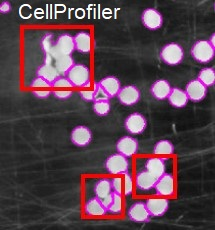
\includegraphics[width=0.48\textwidth]{images/concurrent_meerdere_cellen.jpg}
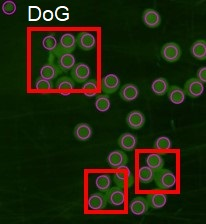
\includegraphics[width=0.473\textwidth]{images/onze_D_DOG_MSER_verschillende_cellen.jpg}
\caption{\label{fig:rand_vs_cirkel_detectie}Randdetectie door CellProfiler tegenover cirkels door Difference of Gaussian}
\end{figure}

\subsubsection{Parameters}
Deze methoden hebben parameters die eerst moeten afgesteld worden. Een kort overzicht welke dit zijn en wat ze doen vermelden we hieronder.

\begin{description}
   \item[De minimale sigma] Deze parameter zal de minimale grootte van een mogelijke detectie beïnvloeden.
   \item[De maximale sigma] Deze parameter zal de maximale grootte van een mogelijke detectie beïnvloeden.
   \item[De threshold] Deze parameter bepaalt de cut-off tussen wat er wel en niet als cel gedetecteerd zal worden.
\end{description}

\paragraph{De Minimale Sigma}
\label{sub:min_sigma}
Aangezien we zeer kleine cellen ook moeten detecteren zullen we deze waarde instellen op 1. Voor DoG en DoH zal dit goede resultaten geven (indien we dit combineren met andere goede parameters) maar voor LoG is deze waarde te klein. Het probleem is dat LoG soms spookcellen zal detecteren. We kunnen dit oplossen door de waarde te verhogen naar 2 of 3. Merk op dat we deze spookcellen ook kunnen verwijderen door de threshold te verhogen, maar dan zullen andere cellen te vaak niet gedetecteerd worden.

\begin{figure}[H]
\centering
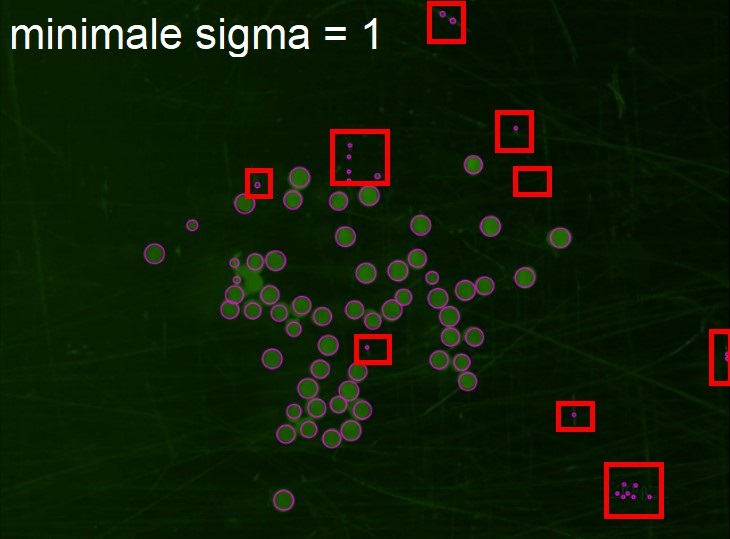
\includegraphics[width=0.98\textwidth]{images/log_spook.jpg}
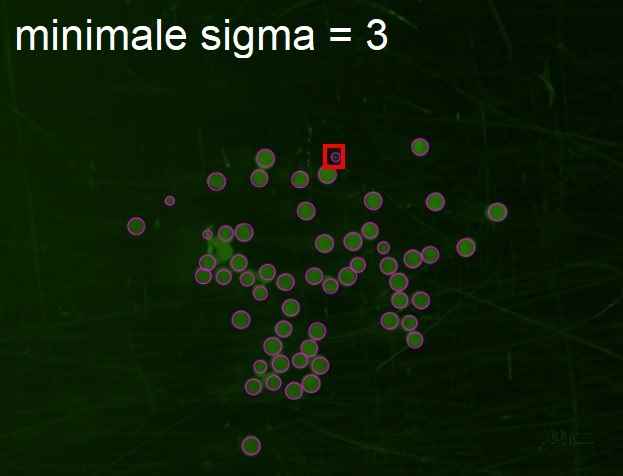
\includegraphics[width=0.98\textwidth]{images/log_geen_spook.jpg}
\caption{\label{fig:spook}LoG met verschillende waarden voor minimale sigma}
\end{figure}


\paragraph{De Maximale Sigma}
\label{sub:max_sigma}
De maximale sigma moet voldoende groot zijn zodat cellen er (bijna) volledig inpassen. Indien dit niet gebeurt, kan het zijn dat een grotere cel als twee cellen gedetecteerd wordt. Indien de maximale sigma te groot wordt, zullen geclusterde cellen als een grote cel gedetecteerd worden. Na vergelijken van verschillende waarden voor sigma besluiten we dat sigma tussen 4 en 8 moet liggen afhankelijk van de datafile. We zullen voor dit project het midden nemen, dus 6. Deze voorwaarde geldt voor DoG, DoH en LoG.

\begin{figure}[H]
\centering
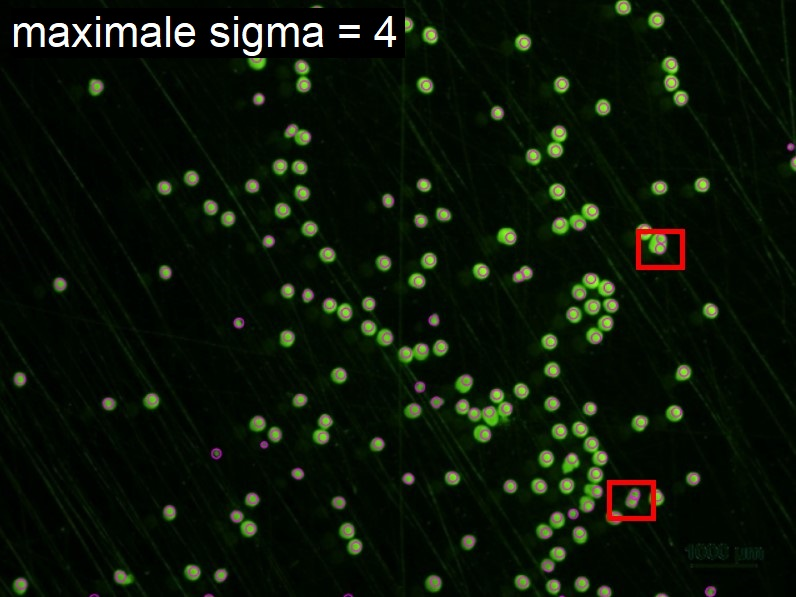
\includegraphics[width=0.98\textwidth]{images/small_sig.jpg}
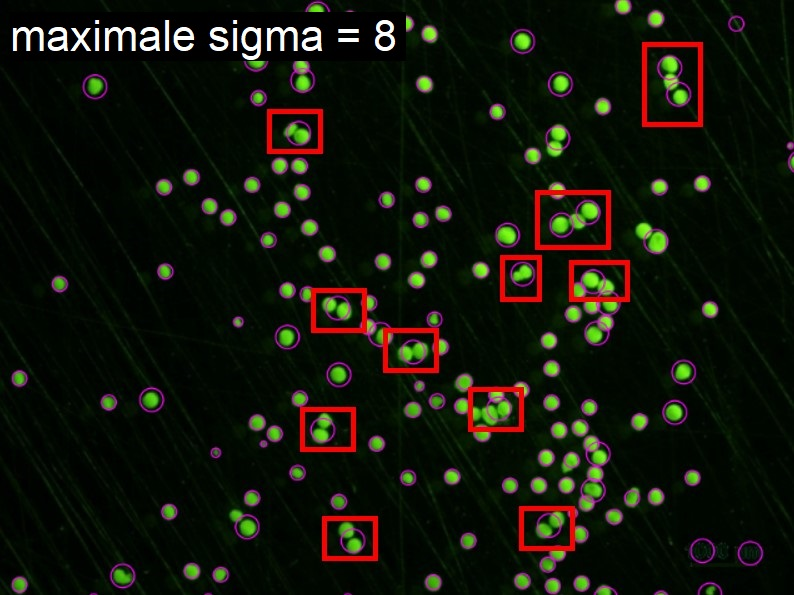
\includegraphics[width=0.98\textwidth]{images/big_sig.jpg}
\caption{\label{fig:max_sigma_bepalen}DoG met verschillende waarden voor maximale sigma}
\end{figure}

\paragraph{De threshold}
Indien de threshold te laag ligt, zullen we vaak ruis detecteren als cel en indien deze te hoog is, zullen er cellen niet gedetecteerd worden. Dit zal vooral voorkomen indien de data veel ruis bevat en er dus minder contrast is tussen ruis en cellen. Voor DoG en LoG moet de threshold tussen 0.06 en 0.11 liggen. Voor DoH geeft geen enkele threshold een goed resultaat indien er veel ruis is. Een goede waarde voor threshold bij DoH is 0.001, andere waarden voor de threshold leveren gelijkaardige of nog slechtere resultaten op. Een threshold hoger dan 0.002 geeft simpelweg geen resultaat.
\begin{figure}[H]
\centering
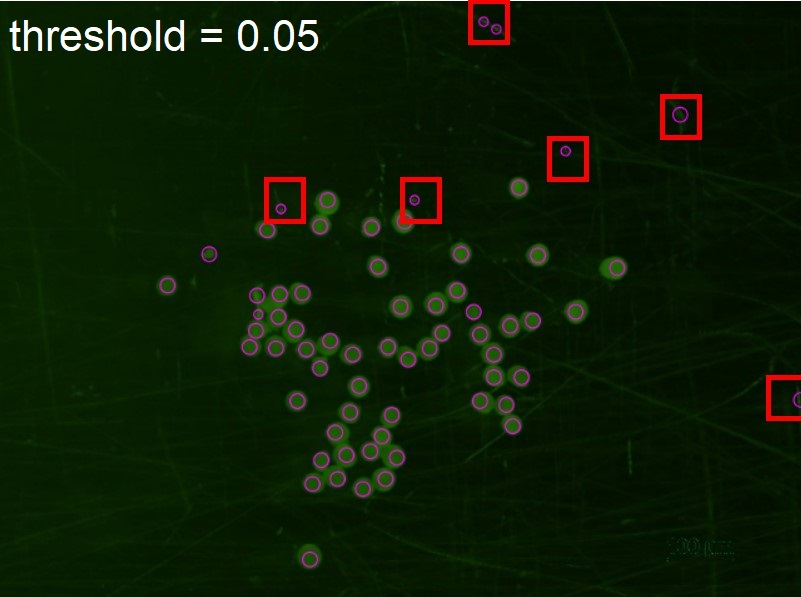
\includegraphics[width=0.89\textwidth]{images/low_threshold.jpg}
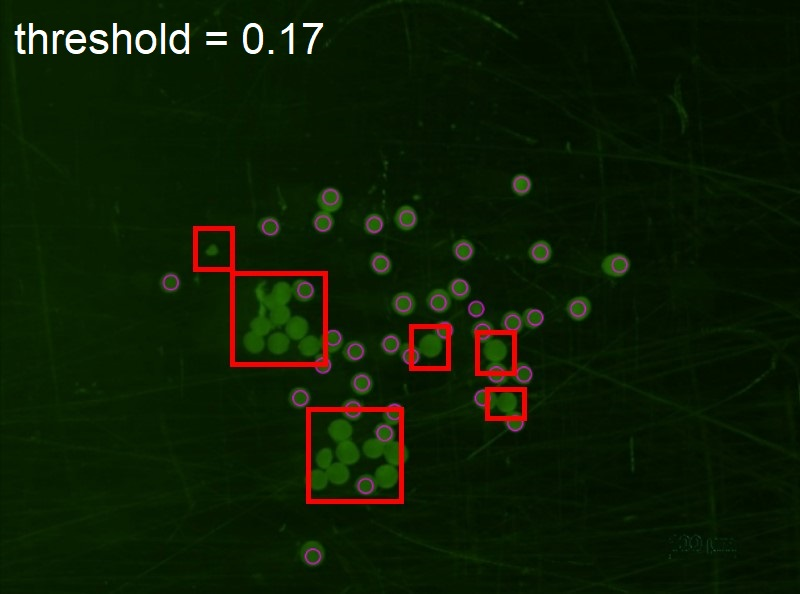
\includegraphics[width=0.89\textwidth]{images/high_threshhold.jpg}
\caption{\label{fig:compare_threshold}DoG met verschillende waarden voor threshold}
\end{figure}

\begin{figure}[H]
\centering
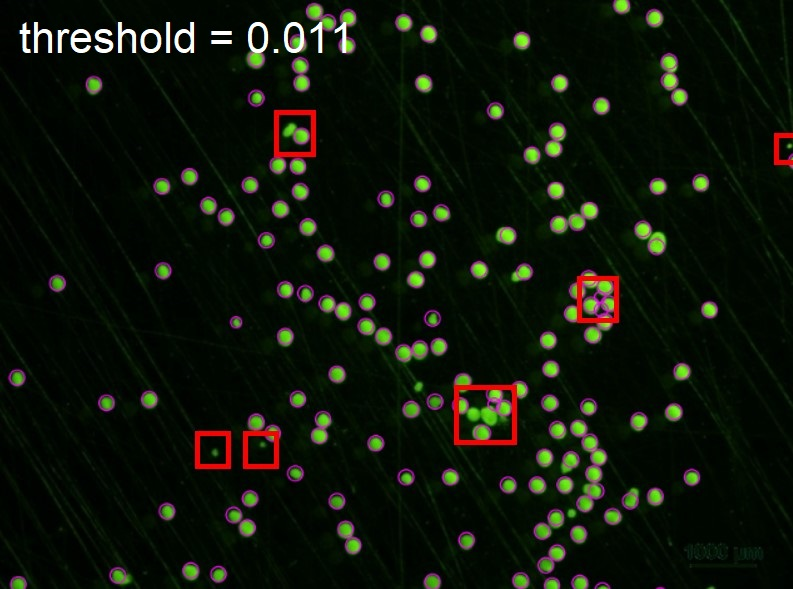
\includegraphics[width=0.89\textwidth]{images/doh_clown_weinig_ruis.jpg}
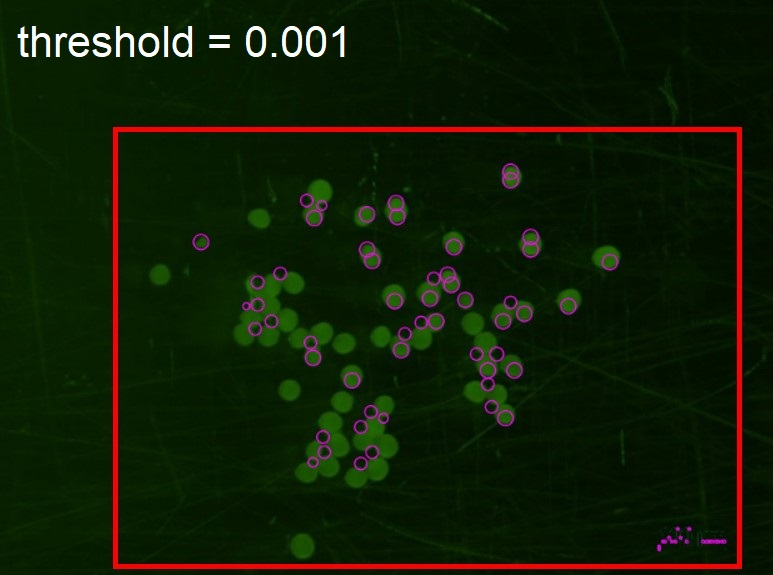
\includegraphics[width=0.89\textwidth]{images/doh_clown.jpg}
\caption{\label{fig:doh_is_clown}DoH met verschillende waarden voor threshold}
\end{figure}


\subsubsection{Overzicht}
We zullen enkel DoG en LoG beschouwen aangezien DoH enkel redelijke resultaten oplevert bij weinig ruis en slechte resultaten bij veel ruis. \\

\autoref{tab:parametersDogLog} geeft goede parameters voor DoG en LoG. Merk op dat dit zeker niet op elke databestand zal werken. Dit komt omdat de gemiddelde en maximale celgrootte verschilt tussen databestanden waardoor parameters niet meer precies zijn. Dit kan opgelost worden door vooraf die beelden te vergroten/verkleinen.
\begin{table}[H]
\begin{tabular}{ |p{1cm}|p{1.5cm}|p{1.5cm}|p{1.5cm}|  }
\hline
 & Minimale sigma & Maximale sigma & Threshold \\
\hline
DoG & 1 & 6 & 0.09 \\
LoG & 3   & 6 & 0.07\\
\hline
\end{tabular}
\caption{Optimale parameters}
\label{tab:parametersDogLog}
\end{table}

\begin{figure}[H]
\centering
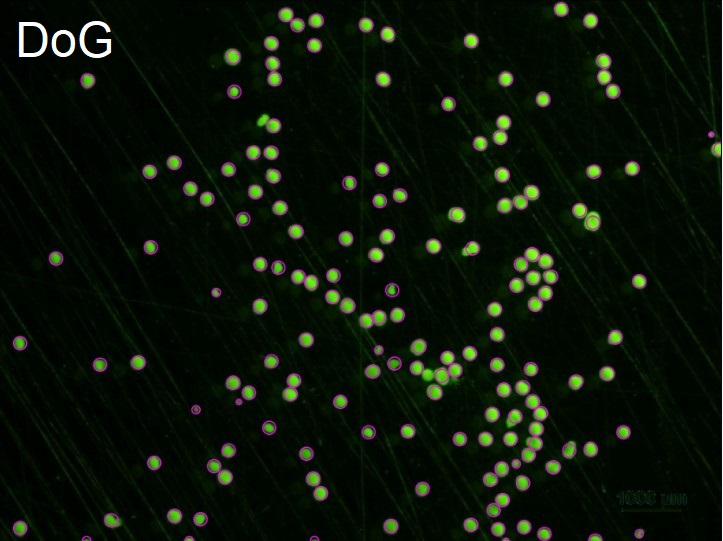
\includegraphics[width=0.98\textwidth]{images/dog_good.jpg}
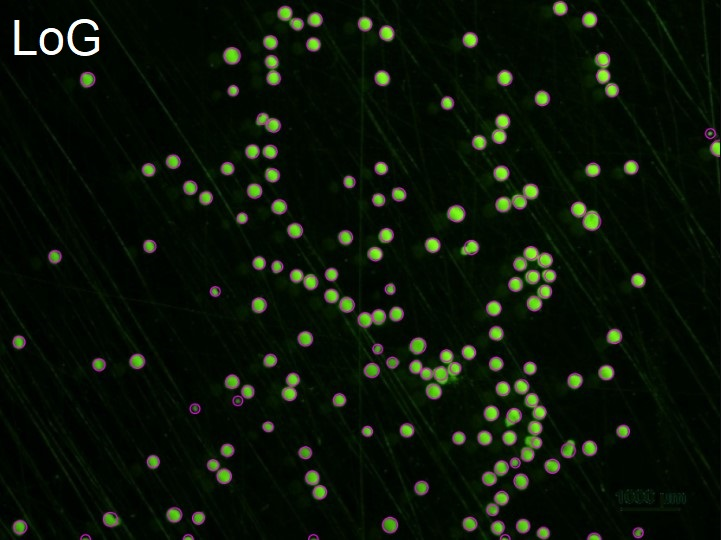
\includegraphics[width=0.98\textwidth]{images/log_good.jpg}
\caption{\label{fig:dog_log_good}DoG en LoG met parameters uit \autoref{tab:parametersDogLog}}
\end{figure}

\subsubsection{Filtering}
In de gebruikte methoden merken we steeds op dat ruis een grote invloed kan hebben op de resultaten. We zullen nu de ruis proberen wegfilteren zonder cellen te verliezen. Dit zal vooral een probleem vormen als de cel heel klein is. Als filtermethode zullen we maximally stable extremal regions (MSER) \cite{ref_MSER} gebruiken. We zullen hier enkel de regio overhouden die relevant is volgens MSER. De rest zal gewoon zwart worden om zo ruis te verwijderen. We willen hiermee de threshold van DoG en LoG verlagen om niet-gedetecteerde cellen toch te kunnen detecteren zonder ruis als cellen aan te zien. Merk op dat de minimale en maximale sigma gelijk zal blijven aangezien de cellen zelf niet zullen verkleinen of vergroten. \\
Voor een goede MSER-filtering zullen we opnieuw de belangrijke parameters goed moeten instellen. Een kort overzicht welke dit zijn en wat ze doen vermelden we hieronder:
\begin{description}
   \item[Delta] Deze parameter kunnen we zien als een threshold en zal beïnvloeden wat er overblijft en wat niet.
   \item[Het minimale gebied] Deze parameter zal bepalen hoe groot een gebied minstens moet zijn om niet gefilterd te worden.
   \item[Het maximale gebied] Deze parameter zal bepalen hoe groot een gebied maximaal mag zijn om niet gefilterd te worden.
\end{description}

\paragraph{Delta}
Een grotere delta zorgt ervoor dat we meer ruis wegfilteren. Indien delta te groot is, zullen ook cellen weggefilterd worden. De waarde moet tussen 4 en 6 liggen, we zullen voor dit project 5 gebruiken.

\begin{figure}[H]
\centering
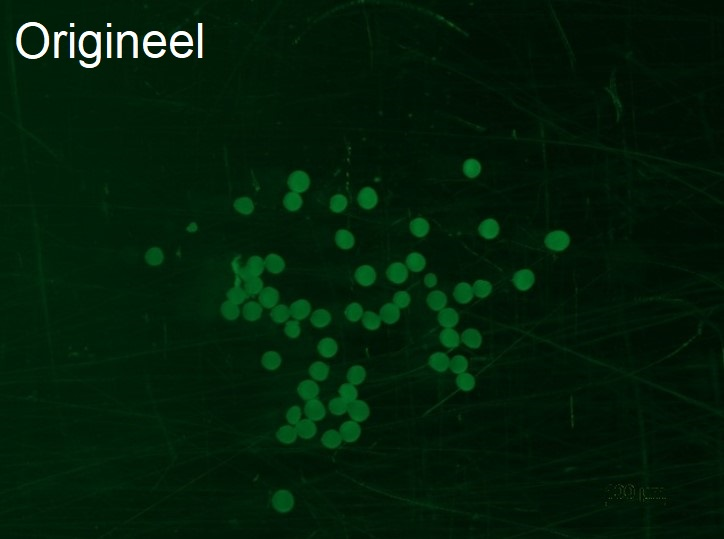
\includegraphics[width=0.98\textwidth]{images/delta_orig.jpg}
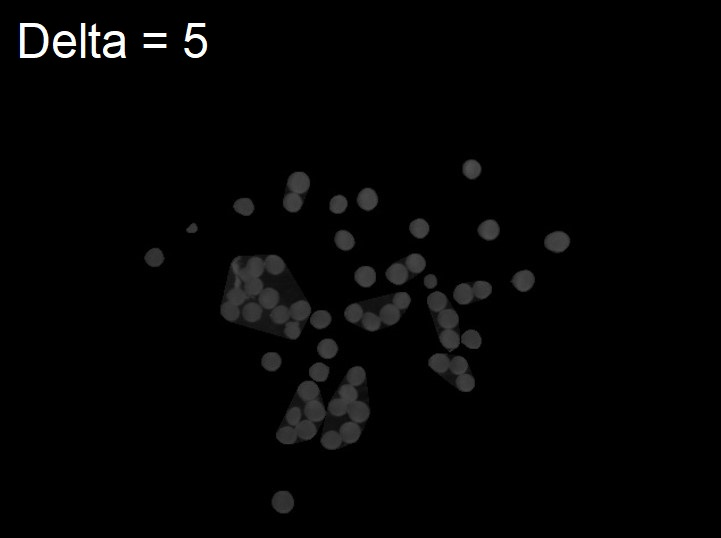
\includegraphics[width=0.98\textwidth]{images/delta_5.jpg}
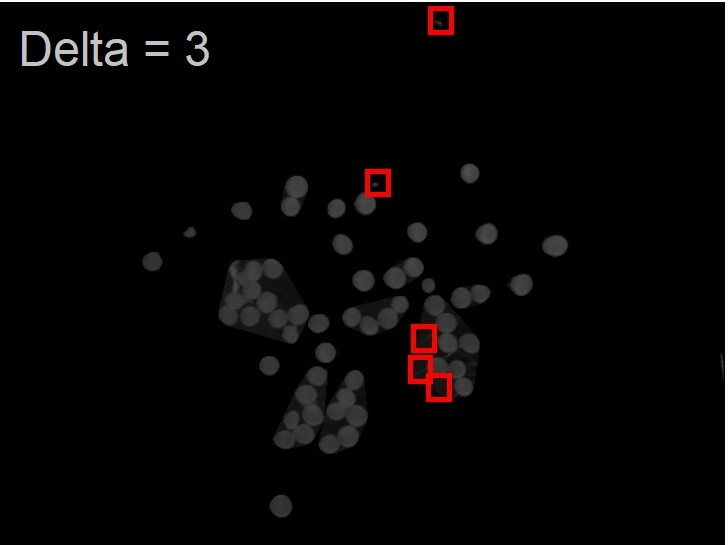
\includegraphics[width=0.98\textwidth]{images/delta_3.jpg}
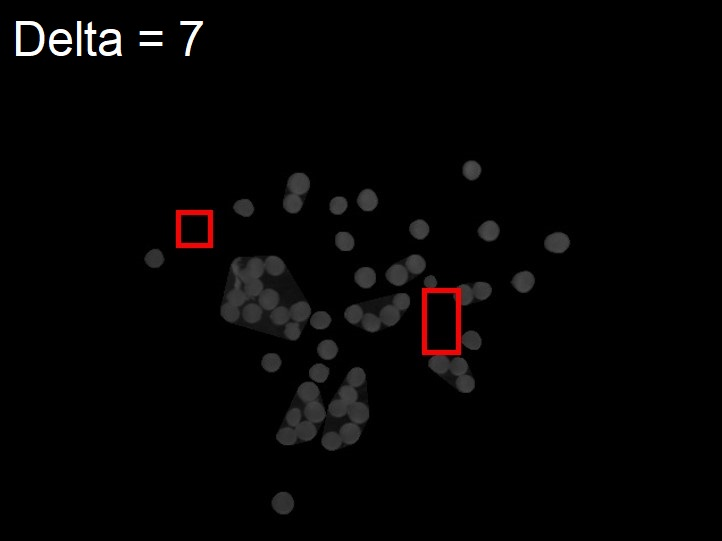
\includegraphics[width=0.98\textwidth]{images/delta_7.jpg}
\caption{\label{fig:delta_mser}Originele afbeelding tegenover MSER-filter toegepast met verschillende waarden voor delta}
\end{figure}

\paragraph{Het minimale gebied}
Het ideale minimale gebied is het gebied dat kleine cellen wel accepteert maar kleine stukjes ruis die een hoge intensiteit hebben niet aanvaardt. Een goede waarde hiervoor ligt tussen 10 en 20, voor dit project zullen we 14 nemen. \autoref{fig:min_area_mser} toont de niet-gefilterde ruis bij minimale gebied = 1.

\begin{figure}[H]
\centering
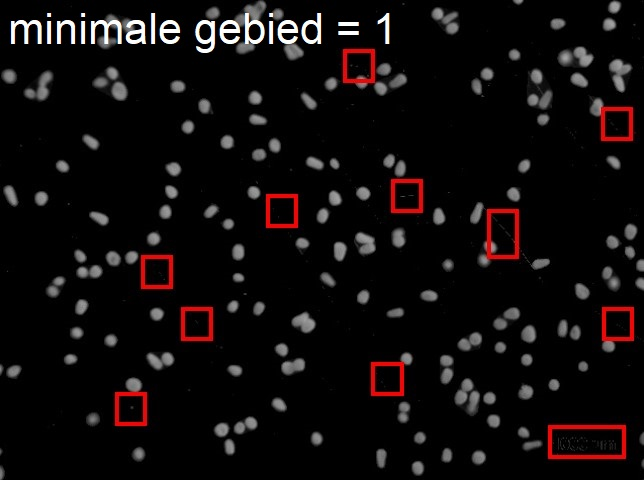
\includegraphics[width=0.98\textwidth]{images/min_area_1.jpg}
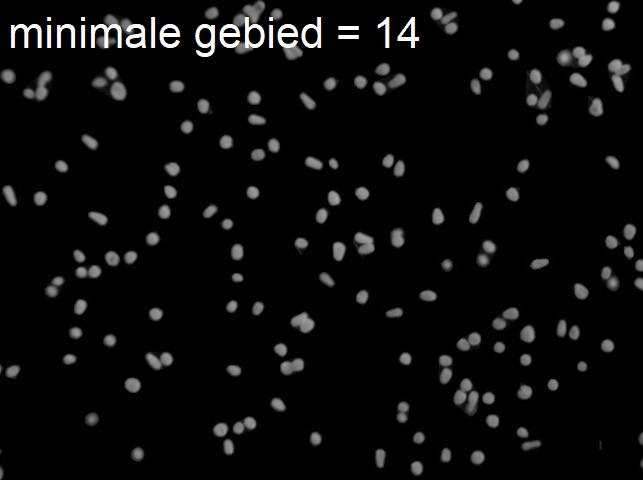
\includegraphics[width=0.98\textwidth]{images/min_area_14.jpg}
\caption{\label{fig:min_area_mser}MSER-filter toegepast met verschillende waarden voor het minimale gebied}
\end{figure}

\paragraph{Het Maximale gebied}
Het maximale gebied moet groot genoeg zijn om geclusterde cellen volledig te omvatten. Indien dit niet gebeurt, zal de volledige cluster wegvallen. Voor dit project zullen we 5000 nemen, maar hogere waarden zullen ook volstaan.

\begin{figure}[H]
\centering
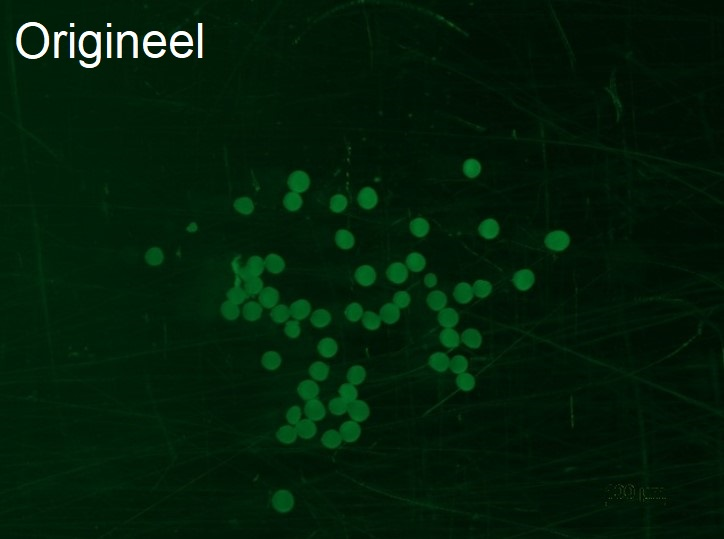
\includegraphics[width=0.98\textwidth]{images/delta_orig.jpg}
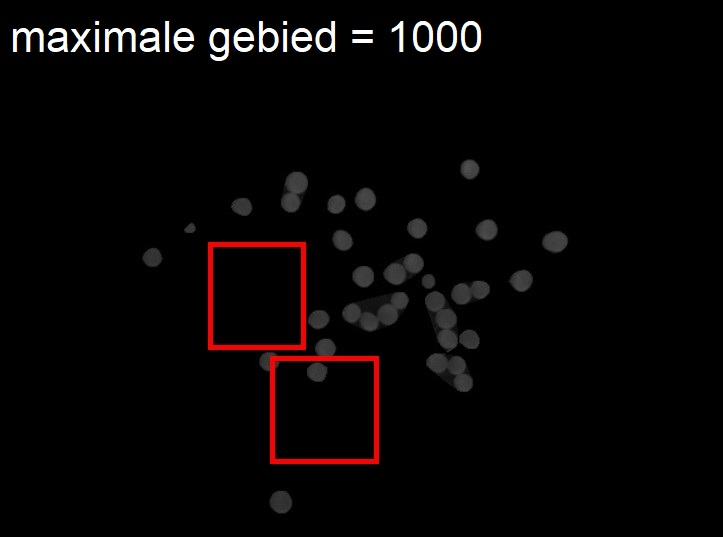
\includegraphics[width=0.98\textwidth]{images/max_area_1000.jpg}
\caption{\label{fig:max_area_mser}Originele afbeelding tegenover MSER-filter toegepast met te klein maximaal gebied}
\end{figure}

\subsubsection{Overzicht MSER}
MSER-filtering geeft meestal een beter resultaat indien er veel ruis is. Hiervoor moeten we wel de threshold verlagen van 0.07/0.09 naar 0.05. Indien niet veel ruis is, zullen we vaak cellen niet meer detecteren. Als voorverwerkingsstap bij DoG en Log zal MSER dus vaak een slechter resultaat opleveren bij deze dataset aangezien de threshold-parameter van DoG en LoG volstaat om het meeste ruis te filteren. We zouden de delta voor MSER kunnen verlagen zodat we minder cellen foutief wegfilteren, maar dan gaan we te veel ruis detecteren. Ook voor DoH zal MSER niet voldoende helpen. We zullen deze voorverwerkingsstap dus niet gebruiken.

De resultaten staan in \autoref{fig:compare_mser}.

\begin{figure}[H]
\centering
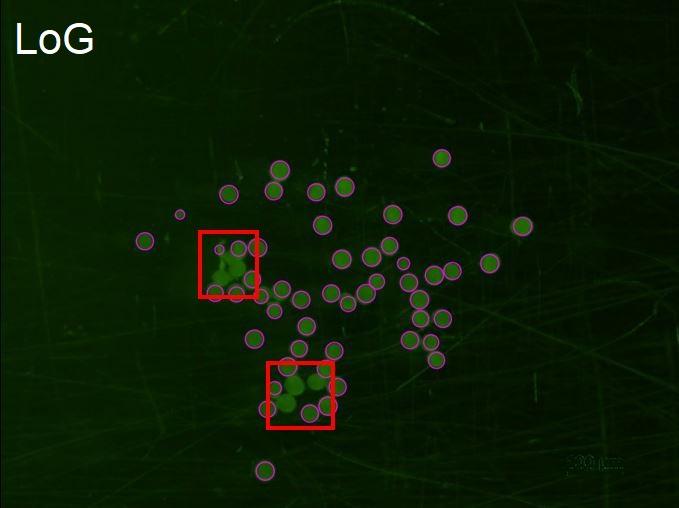
\includegraphics[width=0.98\textwidth]{images/log_no_mser_bad.JPG}
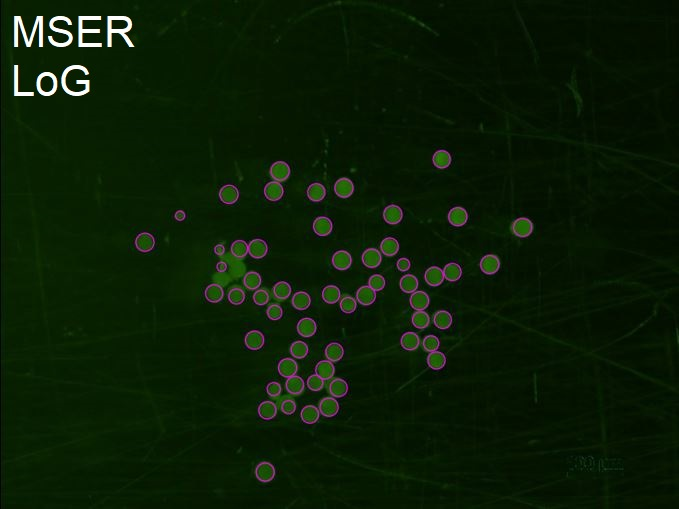
\includegraphics[width=0.98\textwidth]{images/log_mser_good.jpg}
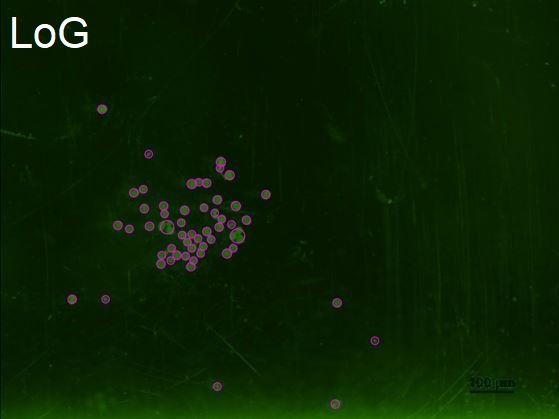
\includegraphics[width=0.98\textwidth]{images/log_no_mser_good.JPG}
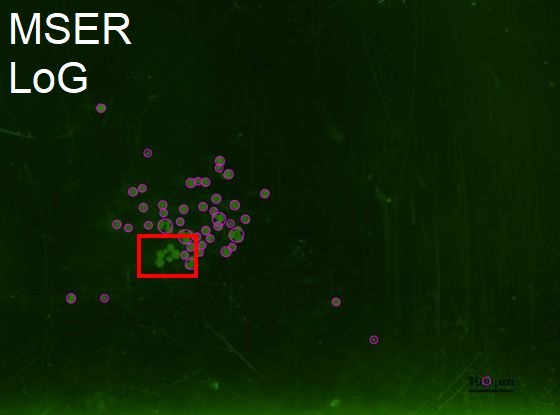
\includegraphics[width=0.98\textwidth]{images/log_mser_bad.JPG}
\caption{\label{fig:compare_mser}De resultaten van het gebruik van MSER-filtering zijn niet consistent}
\end{figure}

Merk op dat op \autoref{fig:compare_mser} subfiguur 3 enkele cellen als groep gedetecteerd worden. Dit kan opgelost worden voor dit specifieke bestand door de minimale sigma uit \autoref{sub:max_sigma} te verkleinen. Echter zullen we dan voor een ander bestand (\autoref{fig:fix_min_sigma}) waar de minimale sigma minstens 6 moet zijn onaanvaardbaar slechte resultaten krijgen.

\begin{figure}[H]
\centering
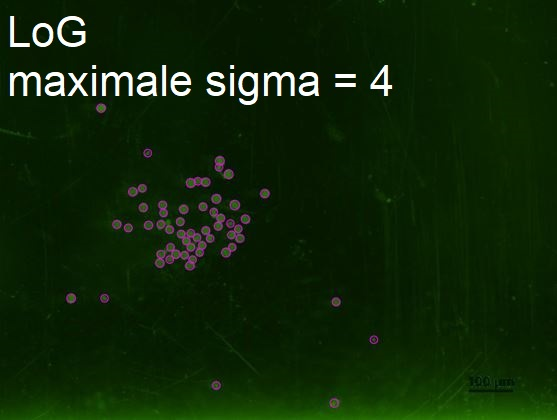
\includegraphics[width=0.98\textwidth]{images/log_fix_min_sigma_good.JPG}
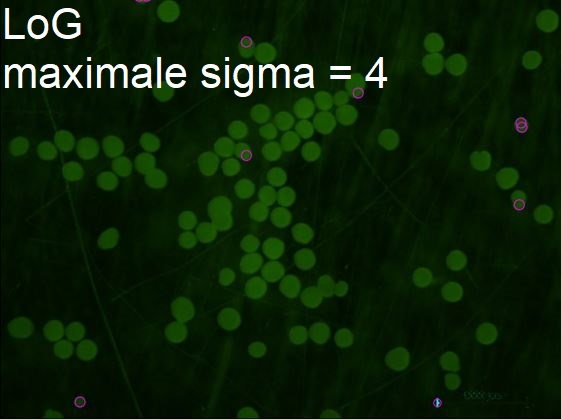
\includegraphics[width=0.98\textwidth]{images/log_fix_min_sigma_bad.JPG}
\caption{\label{fig:fix_min_sigma}De resultaten hangen sterk af van de gemiddelde diameter van de cellen}
\end{figure}

\subsection{Optimale detectie}
\label{sec:optimal_detection}
Onze implementatie van cell tracking zal uiteindelijk LoG zonder MSER gebruiken. In principe kan ook DoG zonder MSER gebruikt worden, daar de precisie vaak vergelijkbaar is.

\section{Optische Flow}
\textit{Opmerking: in dit onderdeel en \autoref{sec:cell_tracking} worden enkel de resultaten besproken van} \verb|A2_mo4_1x_5.avi| \textit{. De conclusie voor de andere data is echter analoog, behalve voor de enkele beelden die op een andere schaal gemaakt zijn. Daar stellen we voor om het beeld te vergroten/verkleinen zodat de diameter van een cel in pixels ongeveer gelijk is aan die in } \verb|A2_mo4_1x_5.avi|.
\newline
\newline
\noindent Optische flow betreft de richting en grootte van de beweging van iedere pixel. Intuïtief komt dit overeen met het volgen van objecten op het beeld. Hiervoor bestaan verschillende methoden en algoritmen \cite{opt_flow_multi_algos}. In dit onderdeel vergelijken we de ideeën van twee algoritmen: Horn–Schunck en Lucas-Kanade. In \autoref{sec:opt_flow_opt_parameters} bespreken we de resultaten na uitvoering met optimale parameters.
\subsection{Horn-Schunck}
Dit is een iteratief algoritme over het volledige beeld. Het is gebaseerd op de veronderstelling dat de luminantie van een object gelijk blijft tussen de twee beelden en dat objecten elastisch zijn en coherent samen bewegen (smoothness).

Stel een functionaal die bestaat uit twee termen: een term die de smoothness berekent, en een term dat het verschil in luminantie berekent. Volgens de veronderstelling van Horn-Schunck (constante luminantie en smoothness) wordt de optische flow dus voorgesteld door het minimaliseren van die functionaal.
\subsubsection{Implementatie}
De implementatie is gebaseerd op \cite{py_optflow_github}. De frames worden eerst door een Gaussische filter gehaald. Deze maakt de beelden zachter en zorgt voor minder extreme sprongen in de optische flow. Daarna wordt iteratief de functionaal geminimaliseerd. Tijdens de berekening van de optische flow tussen twee beelden zijn drie extra parameters vereist.
\begin{description}
   \item{$\boldsymbol\sigma$:} Standaarddeviatie van de Gaussische kernel
   \item{$\boldsymbol\alpha$:} Het gewicht van de smoothness-term in de functionaal. Hoe groter deze waarde, hoe kleiner de lokale verschillen worden. Met andere woorden: de flow wordt vloeiender.
   \item{$\mathbf{n}$:} Het aantal iteraties. Meer iteraties zorgen voor een precieser resultaat maar langere uitvoeringstijd.
\end{description}

\noindent Er wordt dus voor iedere pixel een beweging berekend. We nemen dan het gemiddelde van alle bewegingen die starten binnen een gedetecteerde cel op de beginframe om één uniforme beweging per cel uit te komen.

\subsection{Lucas-Kanade}
De Lucas-Kanademethode \cite{ref_LK} is een veel gebruikte methode voor sparse optische flow schatting. In tegenstelling tot het Horn-Schunck algoritme die het volledige frame nodig heeft, werkt de methode van Lucas-Kanade lokaal. Lucas-Kanade gaat ervan uit dat de verplaatsing binnen die lokale omgeving (window) van een pixel uniform is en lost op basis van deze assumptie de flowvergelijking op voor alle pixels in deze window aan de hand van de kleinste-kwadratenmethode.

\subsubsection{Implementatie}
We gebruikten \verb|calcOpticalFlowPyrLK| uit de opencv-python bibliotheek \cite{ref_opencv_LK}. Dit is een piramidale implementatie \cite{ref_pyr_LK} van Lucas-Kanade die op een recursieve manier beelden van lagere resolutie genereert. Deze beelden worden vervolgens gebruikt om eventuele grote sprongen te kunnen detecteren indien de flow buiten de nabije omgeving van de pixel in kwestie zou vallen.

\begin{figure}[H]
\centering
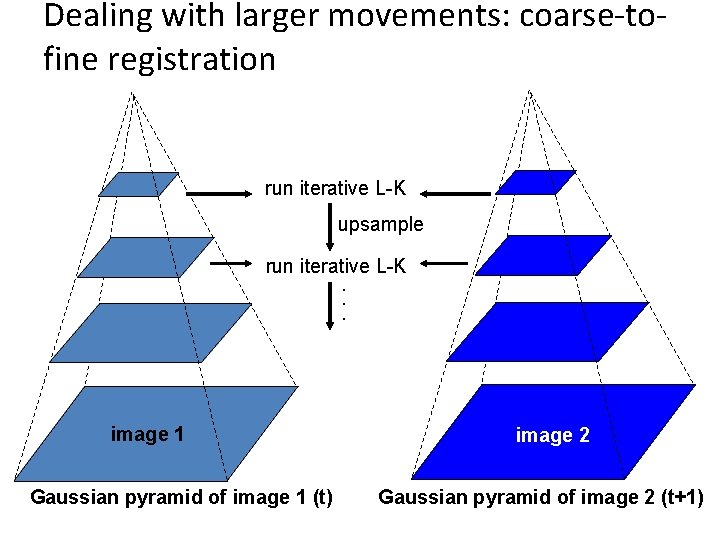
\includegraphics[width=0.98\textwidth]{images/pyr_LK.jpg}
\caption{\label{fig:pyr_LK}Werking van piramidale herschaling van beelden}
\end{figure}

Om deze functie beter te laten werken, zullen dus een aantal parameters goed moeten ingesteld worden.
\begin{description}
   \item[Window size:] Deze parameter zal de grootte van de omgeving rond de pixel in kwestie voorstellen die betrokken wordt bij het berekenen van de verplaatsing.
   \item[Maximal pyramid level:] Deze parameter stelt het maximum aantal recursieve stappen voor die gebruikt worden om het beeld te downscalen.
\end{description}
\subsubsection{Window size}
De window size mag zeker niet kleiner zijn dan de grootste cellen die wij willen volgen. Ook willen we deze zone niet te groot maken aangezien dit tot inaccurate resultaten kan leiden.
\subsubsection{Maximal pyramid level}
Om precisie te bewaren, willen we deze parameter zo klein mogelijk houden. Om eventuele grote sprongen toch te kunnen detecteren, kunnen we dit een beetje vergroten.
\subsubsection{Gekozen regio's}
Zoals eerder vermeld is Lucas-Kanade een sparse methode. Dit betekent dat we regio's moeten opstellen waar het algoritme op moet worden uitgevoerd. Deze regio's bepalen we aan de hand van de Laplacian of Gaussian methode (zie \autoref{sec:optimal_detection}). We stellen de windows dus op rond het middenpunt van iedere cel en bepalen zo per cel in welke richting deze beweegt. Zo hebben we uiteindelijk één uniforme beweging per cel.
\subsubsection{Blurring}
Net zoals bij Horn-Schunck is het mogelijk om een Gaussische filter toe te passen op onze inputbeelden voordat we de Lucas-Kanade methode toepassen.

\subsection{Bepalen optimale parameters}
We willen voor een set van representatieve testdata kijken welk algoritme de minste fouten maakt over de volledige dataset. In tegenstelling tot celdetectie gaan we hier geautomatiseerd en objectief aan de slag. We stellen een scorefunctie op die tracht te evalueren hoe goed een algoritme met bepaalde parameters presteert. Het resultaat van deze scorefunctie lijkt op het principe van een MSE: hoe lager de score, hoe beter het algoritme de optische flow kan berekenen.

Voor beide algoritmen zijn er meerdere parameters die eerst moeten geoptimaliseerd worden. Dit doen we door alle mogelijke combinaties van parameters uit te proberen en deze te evalueren. De combinatie met de laagste score wordt dan gebruikt om de optimale versie van het algoritme voor te stellen in de context van de data.

\subsubsection{Score berekenen}
\label{sec:optflow_score_calc}
De score van één timelapse is de som van de scores van alle paren van opeenvolgende frames. De score van één paar opeenvolgende frames is de som van de evaluatiefunctie $f$ uitgevoerd voor alle pijlen.
Die evaluatiefunctie $f$ heeft twee componenten:
\begin{itemize}
    \item het berekenen van een binaire waarde $b$ die nagaat of de verwachte beweging 'in de buurt ligt van' een gedetecteerde cel uit de volgende frame
    \item het toekennen van een kleine straf indien $b=true$, of het toekennen van een grote straf indien $b=false$
\end{itemize}
Stel $d = $ Euclidische afstand tussen het einde van de pijl en een punt van de omtrek van de cel. 'In de buurt van' wordt hier gedefinieerd als $d$ kleiner is dan 7 pixels.

\noindent Samengevat, \[score = \sum_{pairs}^{}(\sum_{arrows}^{}f(arrow))\]


\subsubsection{Optimale methode en parameters}
\label{sec:opt_flow_opt_parameters}
De optimale parameters voor Horn-Schunck zijn: $\sigma = 5,\ \alpha = 5,\ n = 75$. Een grotere waarde voor $n$ is mogelijk, maar heeft zeer weinig invloed op het resultaat. Enkel de uitvoeringstijd wordt groter.

Voor Lucas-Kanade zijn de parameters: $window size = 15\times15,\ maximal\ pyramid\ level = 2,\ \sigma = 0$. Deze window size komt ongeveer overeen met de grootte van de grotere cellen in de testset, zoals verwacht.
Het is opmerkelijk dat bij Horn-Schunck er wel sterke blur wordt toegepast en bij Lucas-Kanade niet. Als we deze twee methoden met ideale parameters nu tegen elkaar vergelijken, merken we dat Lucas-Kanade ongeveer 10\% lagere scores haalt, en dus beter presteert. Er moet wel context gegeven worden bij deze score: aangezien de meeste cellen amper bewegen, halen beide algoritmen voor die cellen een zeer lage score. Pas bij grote bewegingen zijn er grote verschillen, waarbij Lucas-Kanade veel beter presteert. Daarom zullen we ook die laatste methode gebruiken bij de implementatie van cell tracking. Een ander voordeel van Lucas-Kanade is de uitvoeringstijd. Deze is 5 keer kleiner dan Horn-Schunck met $n = 75$. Door deze snelheid en zeer goede parallellisatiemogelijkheden kunnen we zelfs at-runtime de optimale parameters uitzoeken aan de hand van de scorefunctie. Dit is vooral belangrijk voor $maximal\ pyramid\ level$: we kunnen dus dynamisch datasets met grote en kleine sprongen nog steeds correct interpreteren. Dit heeft minder invloed op de andere parameters, aangezien die afhangen van de parameters van de celdetectie die niet automatisch geoptimaliseerd kunnen worden.

Het dynamisch bepalen van hoe groot $\ maximal\ pyramid\ level$ moet zijn, kan zeer precies verlopen. Door de scorefunctie toe te passen per specifieke cel kan de parameter zich ook aanpassen per berekening per cel. Zo hebben we binnen één overgang dus verschillende waarden voor $\ maximal\ pyramid\ level$.

Doordat Lucas-Kanade lokaal werkt, is het vaak minder verward door omliggende cellen die ook bewegen. Een voorbeeld zien we hiervan in \autoref{fig:optflow_parallel}. De cellen uit de vorige frame zijn paars en de cellen uit de volgende frame zijn groen. De bewegingspijl is rood als de beweging niet in de buurt ligt van een gedetecteerde cel uit de eindframe. Indien wel, dan is de pijl groen. Merk op dat een beweging naar een foute cel uit de eindframe nog steeds groen kan zijn! Dit zien we ook gebeuren in \autoref{fig:optflow_parallel}.
\begin{figure}[H]
\centering
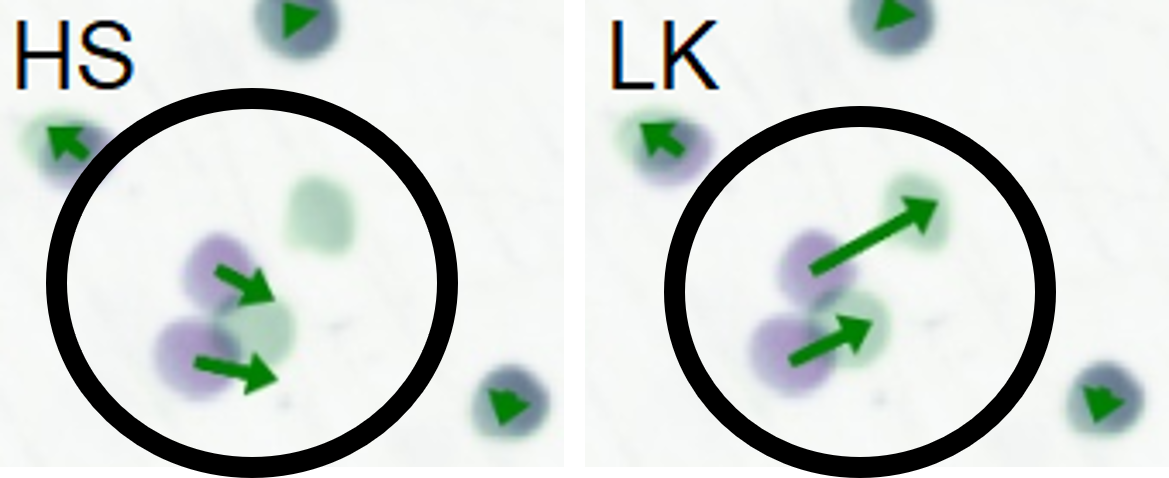
\includegraphics[width=0.98\textwidth]{images/optflow_parallel.png}
\caption{\label{fig:optflow_parallel}Lucas-Kanade werkt beter in een drukke omgeving}
\end{figure}

Ook als we enkele frames laten vallen en de sprongen wat groter worden, blijft Lucas-Kanade de betere methode. In tegenstelling tot \autoref{fig:optflow_parallel} liggen de cellen in \autoref{fig:optflow_grote_sprong} verder van elkaar.
\begin{figure}[H]
\centering
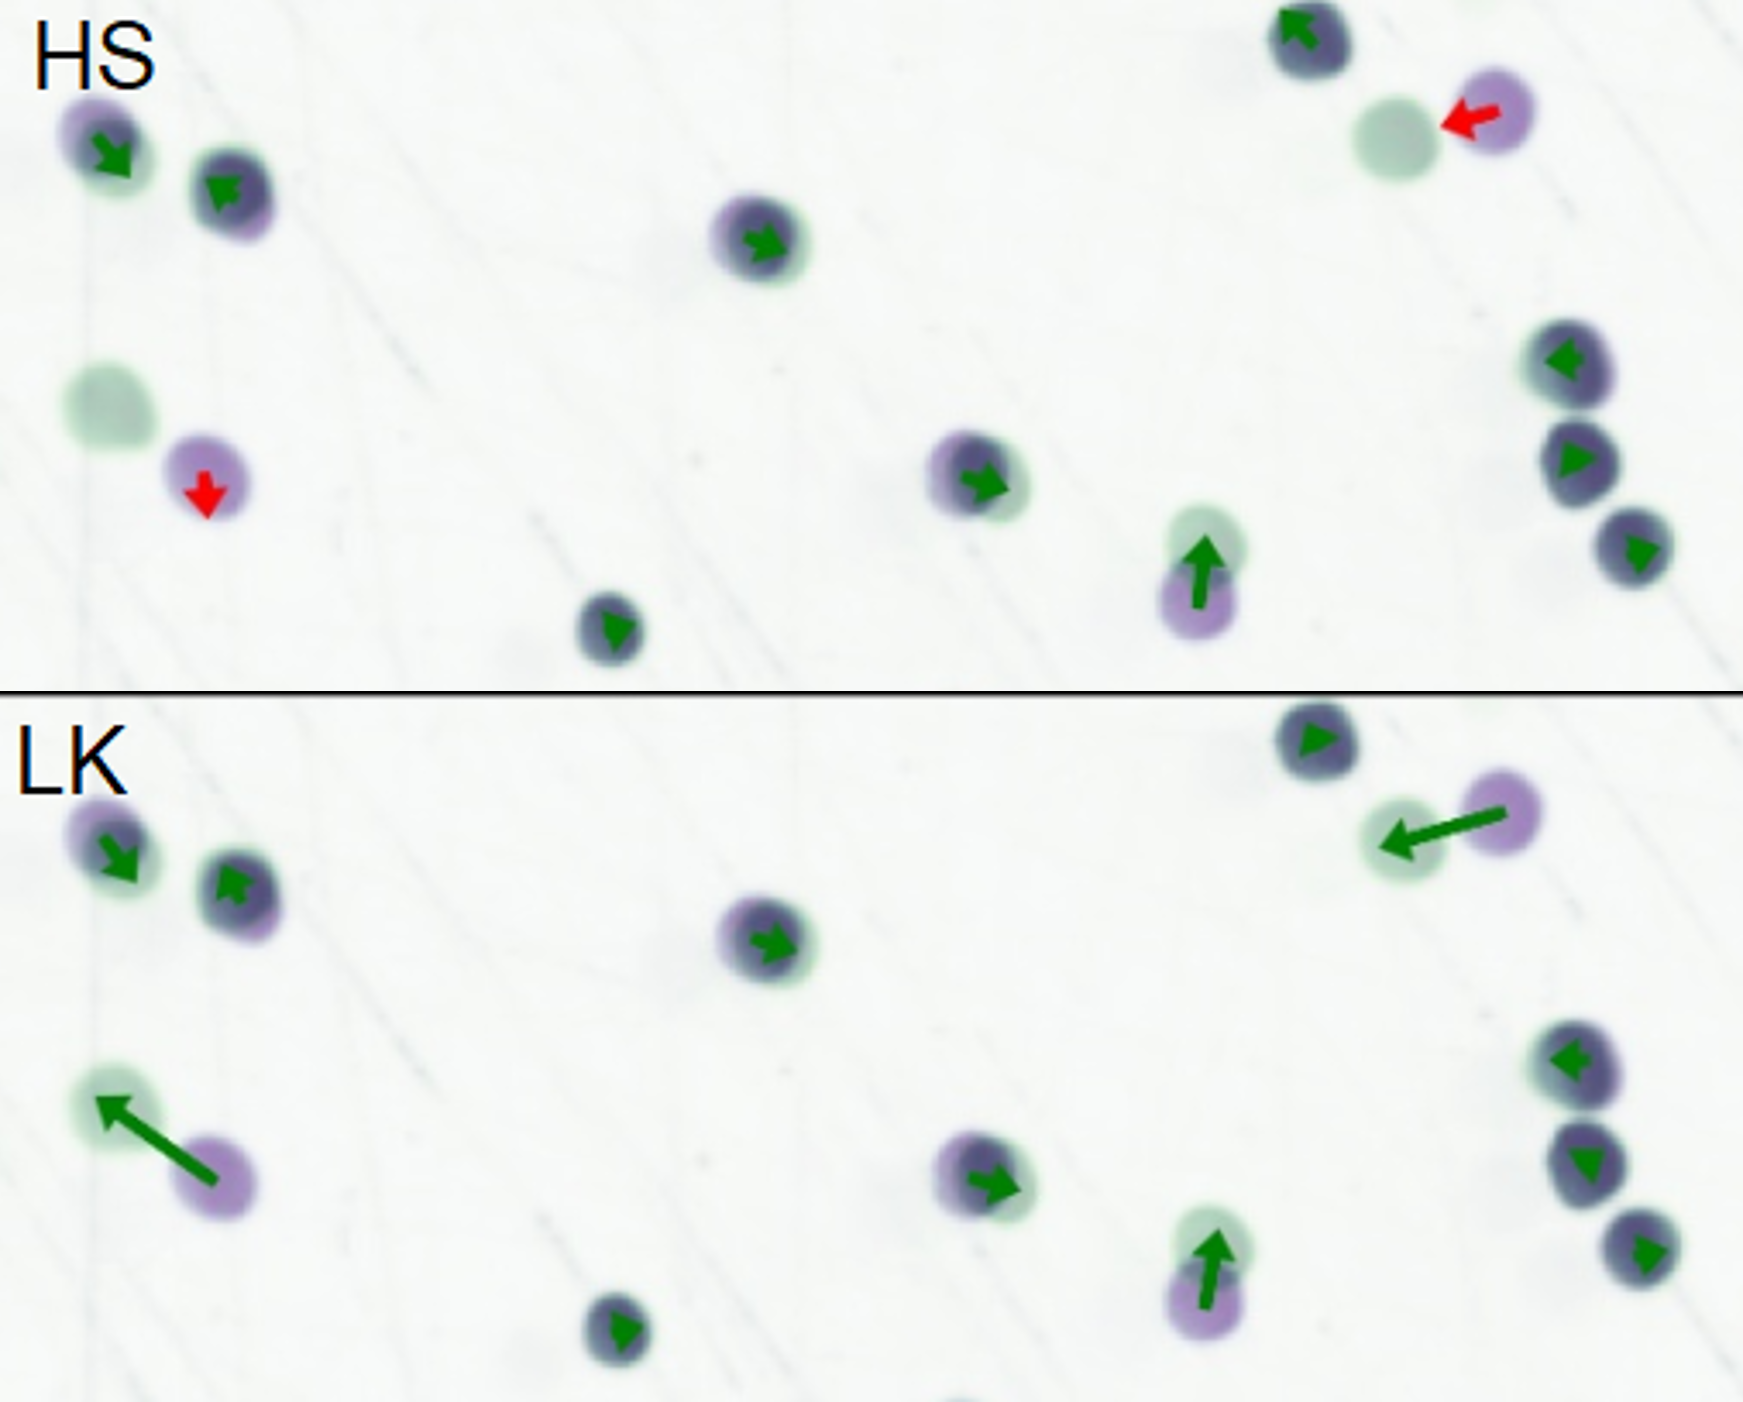
\includegraphics[width=0.98\textwidth]{images/optflow_grotesprong.png}
\caption{\label{fig:optflow_grote_sprong}Lucas-Kanade werkt beter bij grote sprongen}
\end{figure}

\section{Cell tracking}
\label{sec:cell_tracking}
Nu dat we een manier hebben om cellen te detecteren en de verplaatsing tussen twee beelden te berekenen, kunnen we dit gebruiken om het volledige afgelegde pad van een cel te berekenen. We gebruiken Laplacian of Gaussian en Lucas-Kanade zoals vermeld in \autoref{sec:optimal_detection} en \autoref{sec:opt_flow_opt_parameters}.
\subsection{Methode}
Om de paden te berekenen, hebben we natuurlijk eerst de optische flow tussen iedere frame nodig. Dit kunnen we in parallel berekenen aangezien de verplaatsing tussen twee frames onafhankelijk berekend wordt ten opzichte van de verplaatsing tussen twee andere frames. Vervolgens willen we de resulterende flows met elkaar verbinden door de eindcoördinaten van een flow te verbinden met de dichtst bijliggende begincoördinaten van de flow die erop volgt. Analoog aan \autoref{sec:optflow_score_calc} wordt de afstand tussen coördinaten berekend aan de hand van de Euclidische afstand. Indien deze afstand groter is dan 7 pixels, gaan we ervan uit dat de cel niet werd gedetecteerd in de volgende frame en sluiten we het pad af. Indien meerdere cellen aan hetzelfde begincoördinaat verbonden worden, wordt slechts 1 van deze gelinkt en start het andere een nieuw pad. Indien er op het einde van dit zoekproces nog begincoördinaten overblijven, starten deze een nieuw pad. Om het bekomen pad zo vloeiend mogelijk te maken, slaan we enkel de coördinaten op die bekomen zijn door het celdetectiealgoritme in plaats van door het optical flow algoritme. Op het einde van het algoritme bekomen we een lijst van alle paden, waarbij een pad wordt voorgesteld door de bezochte coördinaten van een bepaalde cel en de gedetecteerde grootte in iedere frame. \autoref{fig:TRACK_GOOD} is een voorbeeld van zo'n gedetecteerd pad.
\begin{figure}[H]
\centering
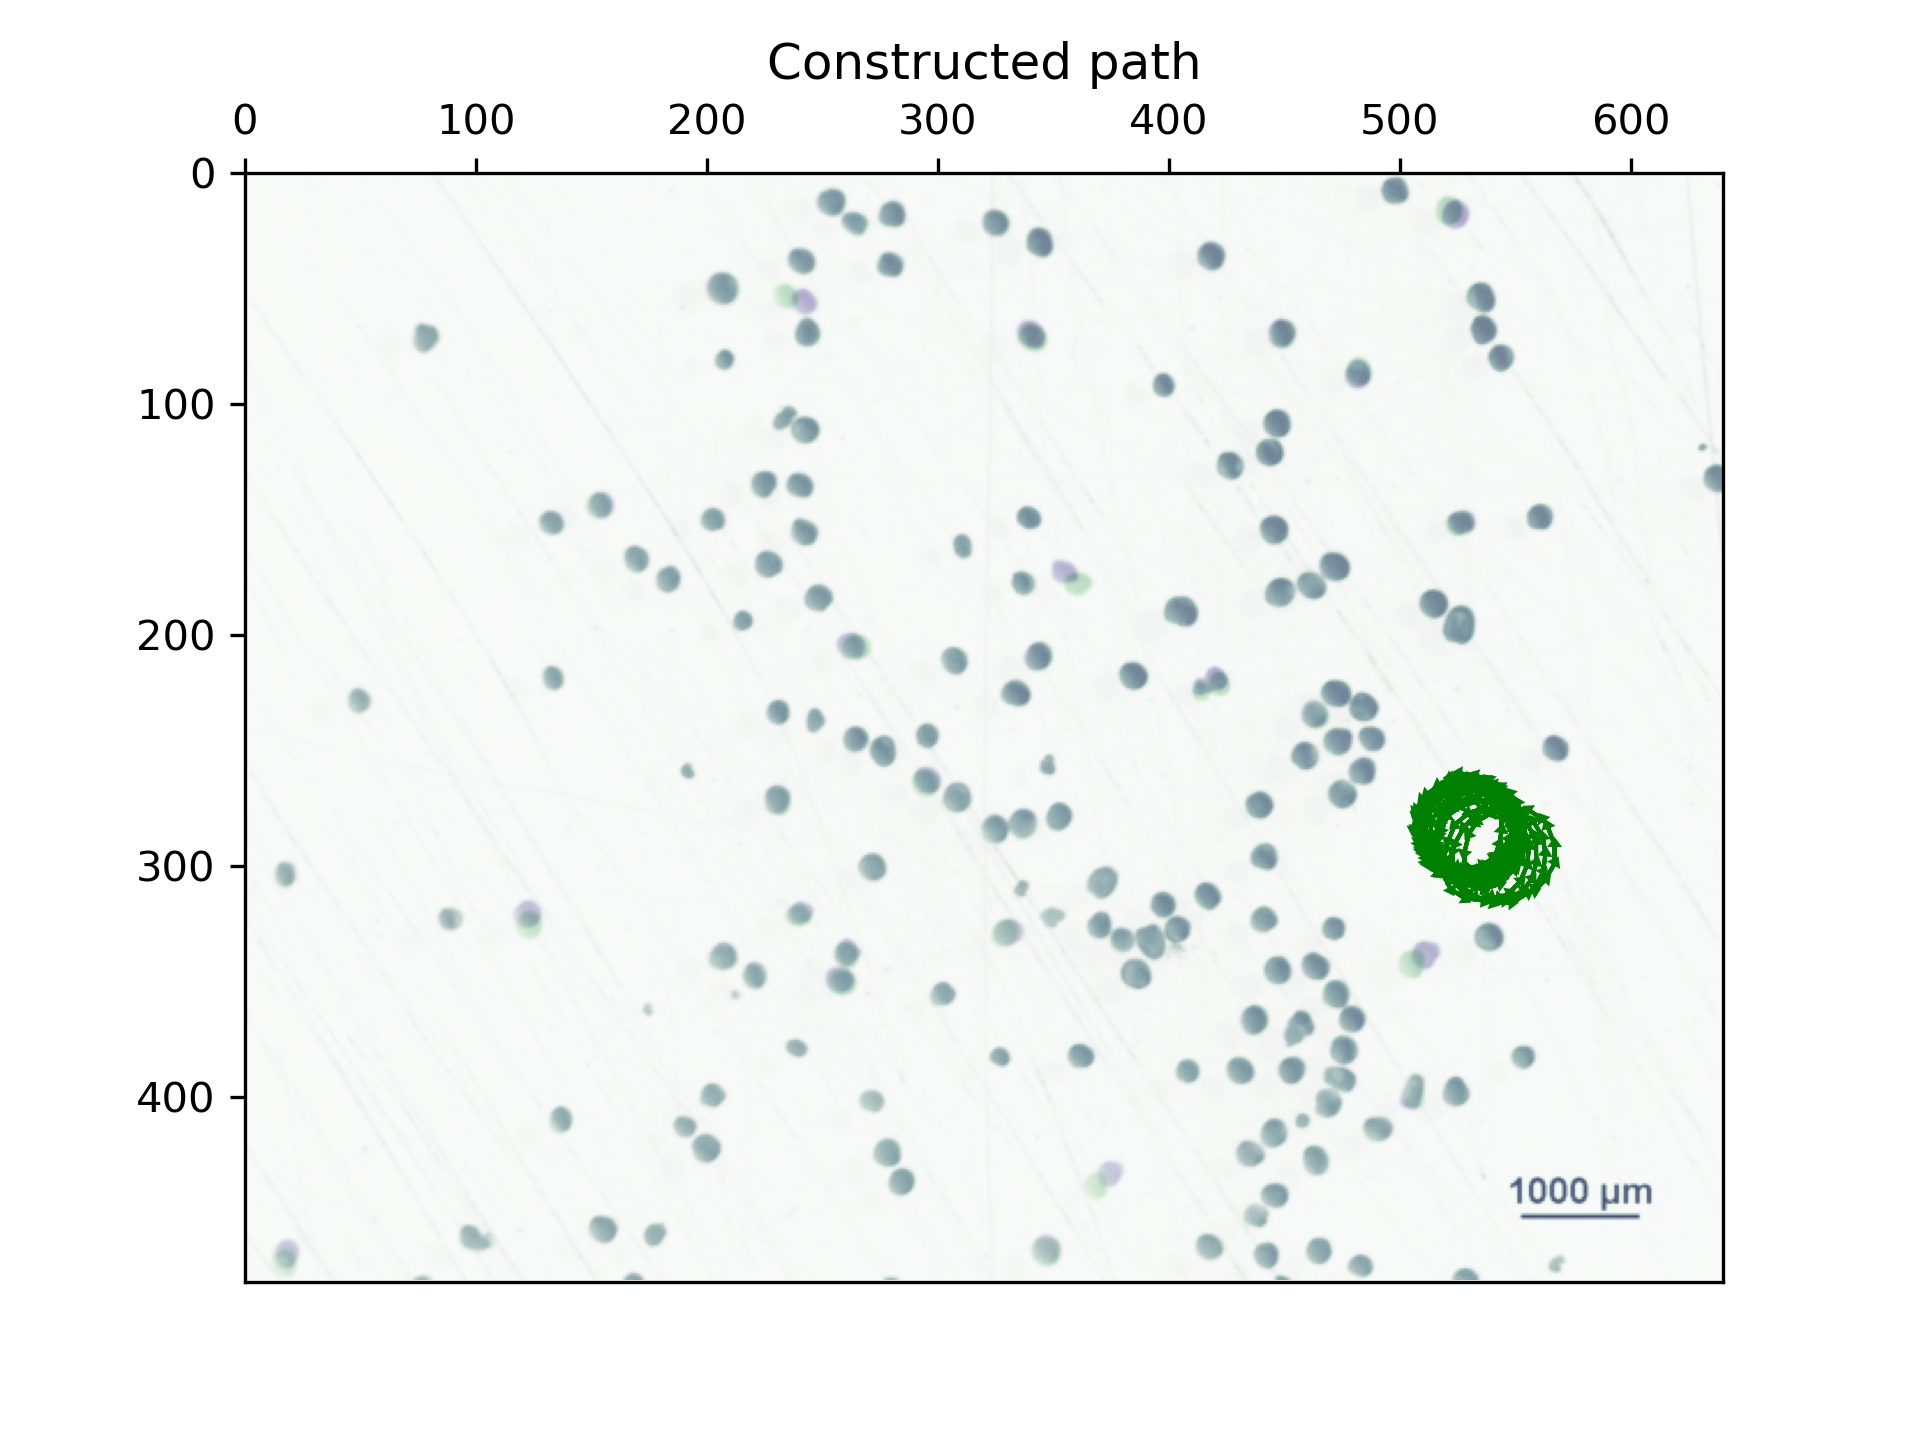
\includegraphics[width=0.98\textwidth]{images/goodpath.jpg}
\caption{\label{fig:TRACK_GOOD}Het gevonden pad van een willekeurige cel getekend}
\end{figure}
\subsection{Problemen met deze aanpak}
\label{sec:tracking_problemen}
Deze methode werkt over het algemeen heel goed als de cellen niet overlappen. Jammer genoeg kunnen we dit niet altijd garanderen en kan het voorvallen dat twee cellen toch overlappen in het beeld. In dat geval is er een kans dat een pad opeens een andere cel begint te volgen en de werkelijke cel achterlaat. Dit komt door de limitaties van de celdetectie bij 2D beelden. Het overige pad dat door de werkelijke cel wordt afgelegd, wordt nog altijd opgeslagen in een nieuw pad, maar wordt niet gelinkt met de voorgeschiedenis. Op \autoref{fig:TRACK_BAD} wordt in het begin een snelle cel gevolgd, maar na overlapping met een trage cel verspringt het pad naar de andere cel en blijft het deze verkeerde cel volgen.

Indien de celdetectie foutief pixels aanduidt als een cel, dan zal ook voor deze ruis een pad berekend worden. Dit zal invloed hebben op de statistieken.
\begin{figure}[H]
\centering
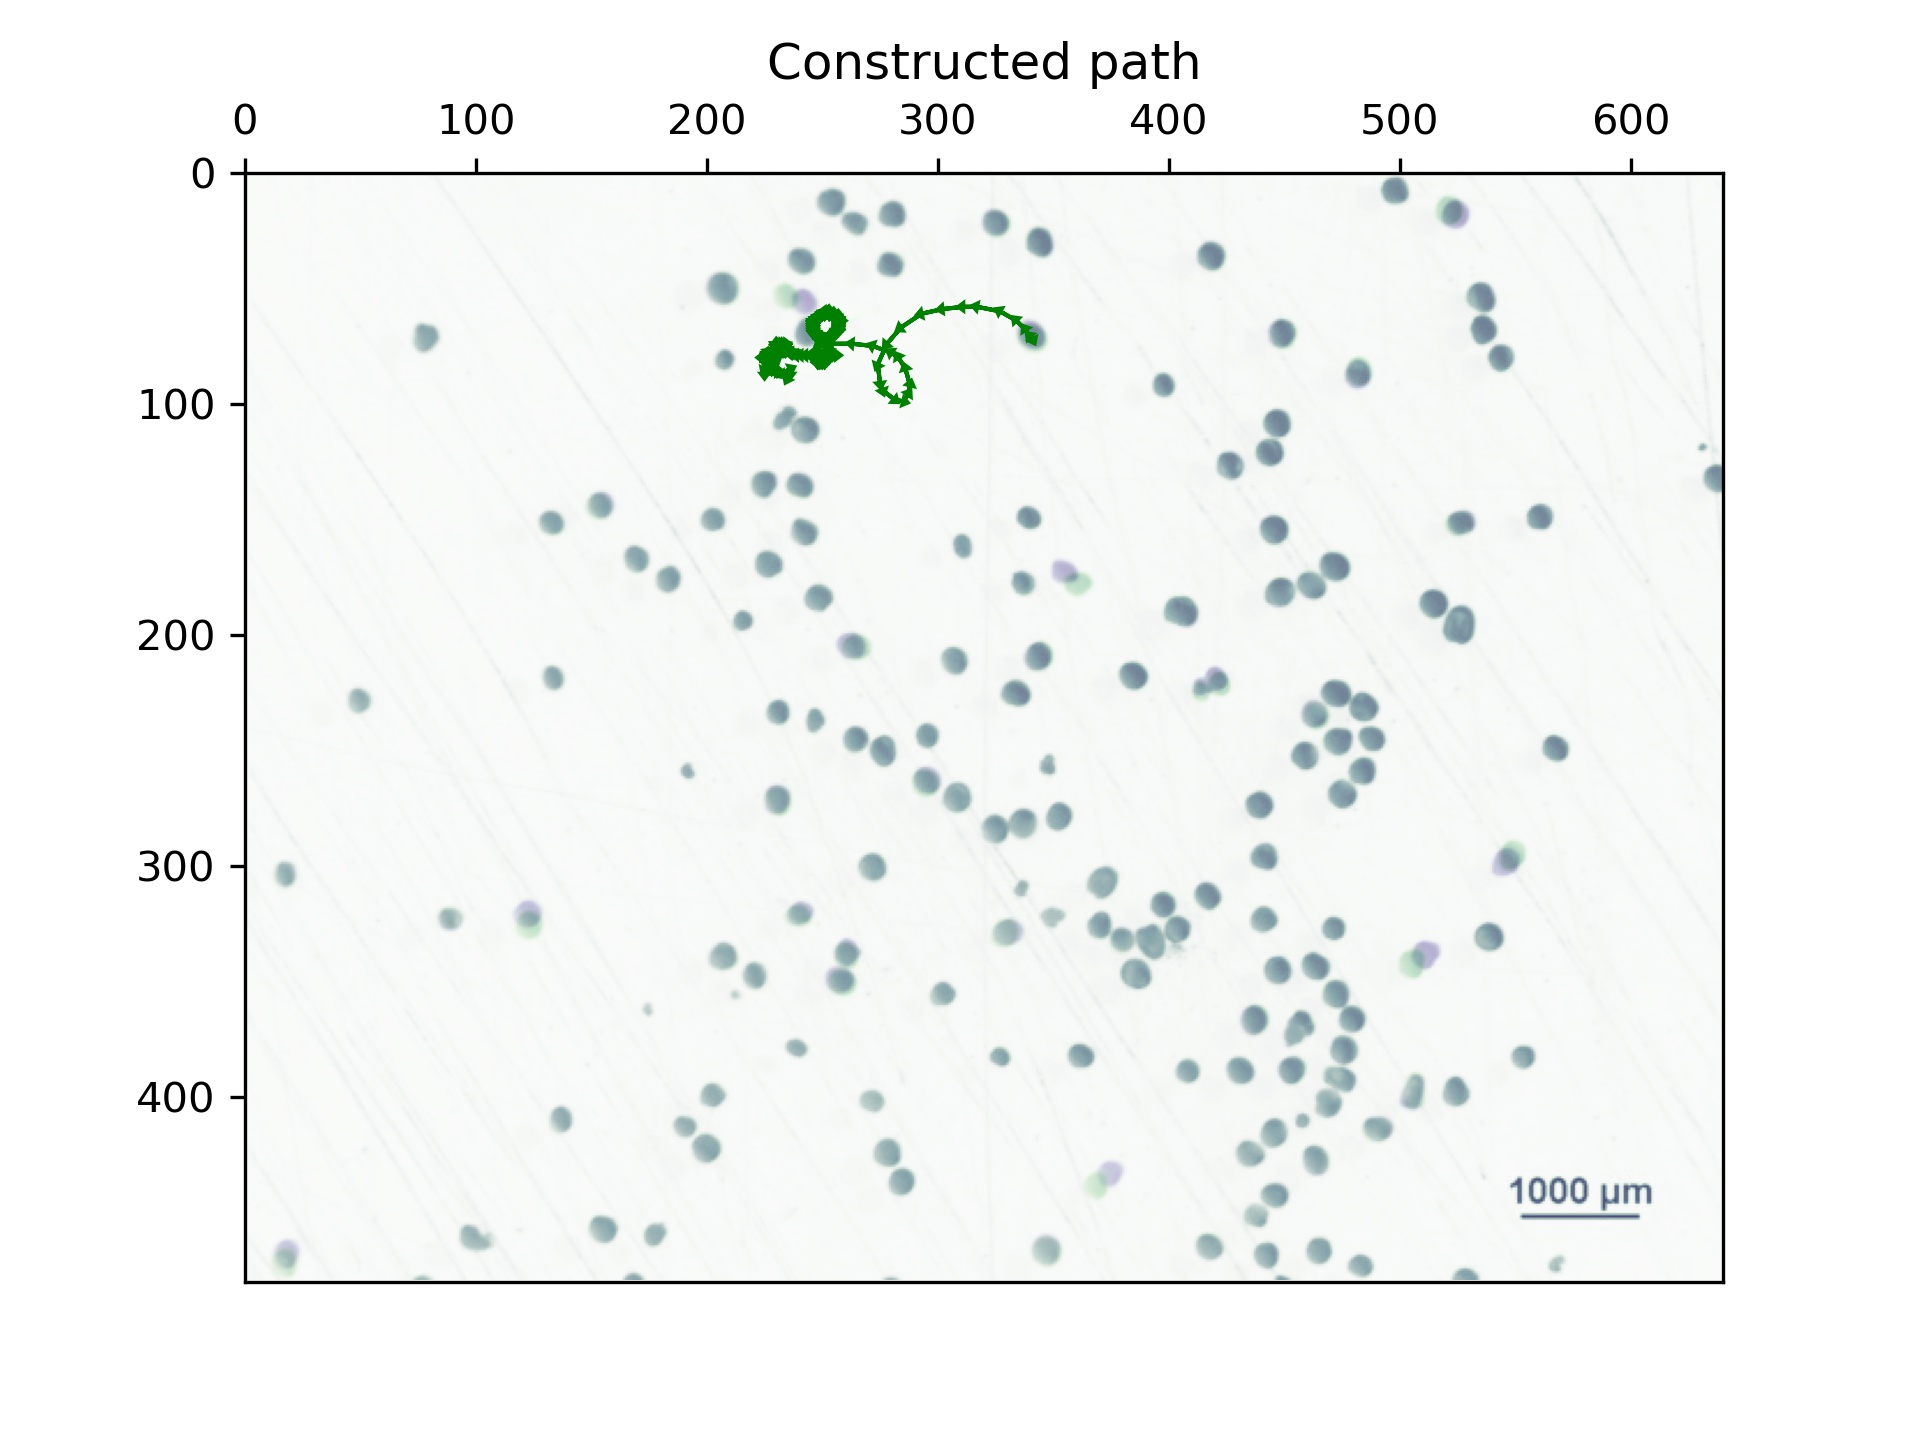
\includegraphics[width=0.98\textwidth]{images/badpath.jpg}
\caption{\label{fig:TRACK_BAD}Pad verspringt van cel na overlap}
\end{figure}
\section{Statistieken}
Met gebruik van de gevonden paden kan men statistieken over de cellen afleiden. In ons onderzoek hebben we bekeken of er een correlatie bestaat tussen de gemiddelde gedetecteerde grootte van een cel en de gemiddelde snelheid van zo'n cel. Deze waarden hebben we geplaatst op \autoref{fig:STATS}.
\begin{figure}[H]
\centering
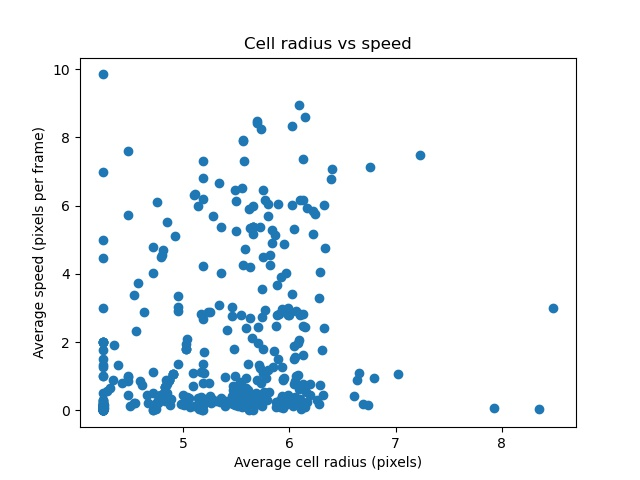
\includegraphics[width=0.98\textwidth]{images/speed.jpg}
\caption{\label{fig:STATS}Gemiddelde straal t.o.v. gemiddelde snelheid van een cel}
\end{figure}
De bekomen Pearson correlatiecoëfficiënt komt neer op $0,250533$ met p-waarde $1,23118\mathrm{e}{-7}$. Hieruit kunnen we afleiden dat er weinig tot geen correlatie tussen deze waarden bestaat en dat deze correlatiecoëfficient statistiek significant is.

\section{Toekomstig Werk}
\subsection{Celgrootte}
Een probleem bij de data is dat de cellen in verschillende video's een verschillende grootte hebben waardoor de maximale sigma uit \autoref{sub:max_sigma} moeilijk vast te leggen is.
Maar aangezien in één video de cellen ongeveer gelijk zijn, zouden we deze kunnen herschalen waardoor we de maximale sigma wel kunnen vastleggen.
\subsection{Overlap}
In \autoref{sec:tracking_problemen} vermelden we reeds de problemen met overlappende cellen: indien cellen overlappen, kan het zijn dat er maar één cel gedetecteerd wordt terwijl dit in de vorige frames nog twee aparte cellen waren. In latere frames, waar ze minder/niet overlappen, zullen we dan weer twee cellen detecteren. Om te achterhalen welk pad overeenkomt met welke cel na de overlap, kunnen we naar meerdere voorgaande frames kijken waar we beide cellen detecteerden. Dan kunnen we op basis van de voorgaande beweging beter voorspellen bij welke cel het pad na overlap hoort.
\section{Conclusie}
We slagen erin om op accurate wijze cellen te detecteren en volgen op microscoopbeelden. Voor celherkenning bekomen we de beste resultaten met Laplacian of Gaussian ($minimale\ sigma = 3,\ maximale\ sigma = 6,\ treshold = 0.07$) en Difference of Gaussians ($minimale\ sigma = 1,\ maximale\ sigma = 6,\ treshold = 0.09$). Voor het berekenen van optische flow geeft Lucas-Kanade ($window\ size = 15\times15,\ maximal\ pyramid\ level = 2,\ \sigma = 0$) betere resultaten dan Horn-Schunck ($\sigma = 5,\ \alpha = 5,\ n = 75$), vooral bij grotere sprongen en drukkere omgevingen. Lucas-Kanade kan de piramidale parameter dynamisch bepalen door verschillende waarden te proberen en het beste resultaat te gebruiken. Door Laplacian of Gaussian te combineren met Lucas-Kanade kunnen cellen op een accurate manier gevolgd worden, met uitzondering op het geval waarbij cellen tijdelijk overlappen.

\nocite{*} % Print de volledige bibliografie
\printbibliography
\end{multicols}
\end{document}
